\documentclass[a4paper,14pt]{extarticle}

\usepackage[T2A]{fontenc}
\usepackage[utf8]{inputenc}
\usepackage[russian]{babel}
\usepackage{amsmath,amssymb}
\usepackage{graphicx}
\usepackage{booktabs}
\usepackage{longtable}
\usepackage{float}
\usepackage{geometry}
\usepackage{caption}
\usepackage{subcaption}
\usepackage{indentfirst}
\usepackage{hyperref}

\geometry{left=25mm,right=15mm,top=20mm,bottom=20mm}
\graphicspath{{../results/plots/}}
\captionsetup{labelsep=period}
\setlength{\parindent}{1.25cm}
\setlength{\parskip}{0pt}

\newcommand{\fro}{\mathrm{F}}
\newcommand{\norm}[1]{\left\lVert #1 \right\rVert}
\newcommand{\secUnit}{с}
\newcommand{\captionNoPivot}{Агрегированные результаты: без выбора ведущего элемента}
\newcommand{\captionRowPivot}{Агрегированные результаты: выбор по строке}
\newcommand{\captionColumnPivot}{Агрегированные результаты: выбор по столбцу}
\newcommand{\captionGlobalPivot}{Агрегированные результаты: глобальный выбор}

\begin{document}

\begin{titlepage}
    \centering
    {\large Лабораторная работа 2\par}
    \vspace{1.5cm}
    {\LARGE\bfseries LU-разложение матрицы Гильберта с использованием MPI\par}
    \vspace{1.0cm}
    {\large Отчет по исследованию параллельных алгоритмов LU-разложения\par}
    \vfill
    {\large Windows 11, Microsoft MPI, MSVC, CMake\par}
    \vspace{0.5cm}
    {\large \today\par}
\end{titlepage}

\tableofcontents
\newpage

\section{Цель работы}

Цель работы заключается в разработке и исследовании параллельной программы LU-разложения матрицы Гильберта с использованием стандарта MPI. В ходе работы необходимо реализовать несколько вариантов выбора ведущего элемента, измерить время выполнения вычислительного ядра, оценить ускорение и эффективность параллельного выполнения, а также проанализировать численную точность получаемого разложения.

\section{Краткая теория LU-разложения}

LU-разложение представляет матрицу $A \in \mathbb{R}^{n \times n}$ в виде произведения нижней треугольной матрицы $L$ и верхней треугольной матрицы $U$:
\begin{equation}
    A = L U.
\end{equation}
В данной работе используется вариант, в котором диагональные элементы матрицы $L$ равны единице. На шаге $k$ вычисляется ведущий элемент $a_{kk}$, после чего для строк $i>k$ определяются множители
\begin{equation}
    l_{ik} = \frac{a_{ik}}{a_{kk}},
\end{equation}
а активная подматрица обновляется по формуле
\begin{equation}
    a_{ij} := a_{ij} - l_{ik} a_{kj}, \quad i,j>k.
\end{equation}

В экспериментах использовалась матрица Гильберта:
\begin{equation}
    A_{ij} = \frac{1}{i+j+1}, \quad i,j = 0,1,\ldots,n-1.
\end{equation}
Матрица Гильберта плохо обусловлена, поэтому она удобна для демонстрации влияния выбора ведущего элемента на численную устойчивость алгоритма.

При наличии перестановок строк и столбцов разложение записывается как
\begin{equation}
    P A Q \approx L U,
\end{equation}
где $P$ --- матрица перестановки строк, а $Q$ --- матрица перестановки столбцов.

Ошибка восстановления вычислялась по относительной норме Фробениуса:
\begin{equation}
    \varepsilon_{LU} = \frac{\norm{P A Q - L U}_{\fro}}{\norm{A}_{\fro}}.
\end{equation}
Для оценки качества решения также рассматривалась тестовая система $Ax=b$, где истинное решение $x_{true}$ является вектором из единиц, а $b = A x_{true}$. Относительная невязка вычислялась как
\begin{equation}
    r = \frac{\norm{Ax-b}_2}{\norm{b}_2}.
\end{equation}

\section{Описание MPI-распараллеливания}

Параллельная программа использует распределение строк матрицы между MPI-процессами. Для строки с индексом $i$ владелец определяется правилом
\begin{equation}
    owner(i) = i \bmod p,
\end{equation}
где $p$ --- число MPI-процессов. Такое циклическое распределение позволяет достаточно равномерно распределить строки между процессами.

На каждом шаге $k$ процесс-владелец ведущей строки рассылает ее всем процессам с помощью \texttt{MPI\_Bcast}. После этого каждый процесс обновляет только принадлежащие ему строки активной подматрицы. Время измеряется только для вычислительного ядра LU-разложения: перед началом измерения выполняется \texttt{MPI\_Barrier}, а время берется через \texttt{MPI\_Wtime}.

\section{Варианты выбора ведущего элемента}

\subsection{Без выбора ведущего элемента}

В базовом варианте ведущим элементом на шаге $k$ считается текущий диагональный элемент $a_{kk}$. Перестановки строк и столбцов не выполняются, поэтому $P=I$ и $Q=I$. Этот вариант имеет минимальные коммуникационные расходы, но является наименее устойчивым для плохо обусловленных матриц.

\subsection{Выбор по строке}

При выборе по строке на шаге $k$ ищется столбец
\begin{equation}
    pivot\_col = \arg\max_{j=k,\ldots,n-1} |a_{kj}|.
\end{equation}
Затем столбцы $k$ и $pivot\_col$ меняются местами. Программа хранит перестановку столбцов $Q$, а ошибка восстановления считается как $\norm{AQ-LU}_{\fro}/\norm{A}_{\fro}$.

\subsection{Выбор по столбцу}

При выборе по столбцу на шаге $k$ ищется строка
\begin{equation}
    pivot\_row = \arg\max_{i=k,\ldots,n-1} |a_{ik}|.
\end{equation}
Каждый MPI-процесс ищет локальный максимум только среди принадлежащих ему строк, после чего глобальный максимум определяется с помощью \texttt{MPI\_Allreduce}. Если строки принадлежат разным процессам, их обмен выполняется через \texttt{MPI\_Sendrecv}, что исключает взаимную блокировку. Программа хранит перестановку строк $P$, а ошибка восстановления считается как $\norm{PA-LU}_{\fro}/\norm{A}_{\fro}$.

\subsection{Глобальный выбор}

При глобальном выборе на шаге $k$ максимум ищется во всей активной подматрице:
\begin{equation}
    (pivot\_row,pivot\_col) = \arg\max_{i,j=k,\ldots,n-1} |a_{ij}|.
\end{equation}
Глобальный максимум находится параллельно с использованием MPI-редукции по структуре \texttt{value,row,col}. После выбора элемента выполняются и перестановка строк, и перестановка столбцов. В этом случае хранятся обе перестановки $P$ и $Q$, а ошибка восстановления вычисляется как $\norm{PAQ-LU}_{\fro}/\norm{A}_{\fro}$.

\section{Экспериментальная среда}

Эксперименты выполнялись в следующей среде:
\begin{itemize}
    \item операционная система: Windows 11;
    \item MPI-библиотека: Microsoft MPI;
    \item компилятор: MSVC;
    \item система сборки: CMake;
    \item запуск параллельных программ: \texttt{mpiexec};
    \item размеры матрицы: $n = 10, 50, 100, 500, 1000$;
    \item число процессов: $p = 1,2,4,8$;
    \item число повторов для каждого эксперимента: 5;
    \item агрегирование времени: медиана по повторам.
\end{itemize}

Ускорение и эффективность вычислялись по формулам
\begin{equation}
    S_p = \frac{T_1}{T_p}, \qquad E_p = \frac{S_p}{p},
\end{equation}
где $T_1$ --- медианное время выполнения на одном процессе, а $T_p$ --- медианное время выполнения на $p$ процессах для того же алгоритма и размера матрицы.

\section{Результаты экспериментов}

В таблицах \ref{tab:no}--\ref{tab:global} представлены агрегированные результаты из файла \texttt{results\_lu\_agg.csv}. Время указано с шестью знаками после запятой, ускорение и эффективность --- с тремя знаками после запятой, ошибки --- в экспоненциальной форме с тремя знаками после запятой.

\scriptsize
\begin{longtable}{rrrrrrr}
\caption{\captionNoPivot}\label{tab:no}\\
\toprule
$n$ & $p$ & $t$, \secUnit & $S_p$ & $E_p$ & $\varepsilon_{LU}$ & $r$ \\
\midrule
\endfirsthead
\toprule
$n$ & $p$ & $t$, \secUnit & $S_p$ & $E_p$ & $\varepsilon_{LU}$ & $r$ \\
\midrule
\endhead
10 & 1 & 0.000001 & 1.000 & 1.000 & 3.320e-17 & 6.237e-17 \\
10 & 2 & 0.000008 & 0.098 & 0.049 & 3.320e-17 & 6.237e-17 \\
10 & 4 & 0.000005 & 0.167 & 0.042 & 3.320e-17 & 6.237e-17 \\
10 & 8 & 0.005716 & 0.000 & 0.000 & 3.320e-17 & 6.237e-17 \\
50 & 1 & 0.000015 & 1.000 & 1.000 & 8.581e-17 & 2.054e-15 \\
50 & 2 & 0.000040 & 0.378 & 0.189 & 8.581e-17 & 2.054e-15 \\
50 & 4 & 0.000053 & 0.287 & 0.072 & 8.581e-17 & 2.054e-15 \\
50 & 8 & 0.000096 & 0.160 & 0.020 & 8.581e-17 & 2.054e-15 \\
100 & 1 & 0.000090 & 1.000 & 1.000 & 1.183e-16 & 7.079e-16 \\
100 & 2 & 0.000119 & 0.758 & 0.379 & 1.183e-16 & 7.079e-16 \\
100 & 4 & 0.000086 & 1.047 & 0.262 & 1.183e-16 & 7.079e-16 \\
100 & 8 & 0.000163 & 0.554 & 0.069 & 1.183e-16 & 7.079e-16 \\
500 & 1 & 0.011438 & 1.000 & 1.000 & 2.388e-16 & 4.808e-15 \\
500 & 2 & 0.006349 & 1.801 & 0.901 & 2.388e-16 & 4.808e-15 \\
500 & 4 & 0.003984 & 2.871 & 0.718 & 2.388e-16 & 4.808e-15 \\
500 & 8 & 0.004479 & 2.553 & 0.319 & 2.388e-16 & 4.808e-15 \\
1000 & 1 & 0.108050 & 1.000 & 1.000 & 3.228e-16 & 8.490e-15 \\
1000 & 2 & 0.064124 & 1.685 & 0.843 & 3.228e-16 & 8.490e-15 \\
1000 & 4 & 0.052428 & 2.061 & 0.515 & 3.228e-16 & 8.490e-15 \\
1000 & 8 & 0.098542 & 1.096 & 0.137 & 3.228e-16 & 8.490e-15 \\
\bottomrule
\end{longtable}

\begin{longtable}{rrrrrrr}
\caption{\captionRowPivot}\label{tab:row}\\
\toprule
$n$ & $p$ & $t$, \secUnit & $S_p$ & $E_p$ & $\varepsilon_{LU}$ & $r$ \\
\midrule
\endfirsthead
\toprule
$n$ & $p$ & $t$, \secUnit & $S_p$ & $E_p$ & $\varepsilon_{LU}$ & $r$ \\
\midrule
\endhead
10 & 1 & 0.000001 & 1.000 & 1.000 & 4.680e-17 & 1.202e-16 \\
10 & 2 & 0.000008 & 0.111 & 0.056 & 4.680e-17 & 1.202e-16 \\
10 & 4 & 0.000014 & 0.063 & 0.016 & 4.680e-17 & 1.202e-16 \\
10 & 8 & 0.000022 & 0.042 & 0.005 & 4.680e-17 & 1.202e-16 \\
50 & 1 & 0.000018 & 1.000 & 1.000 & 9.728e-17 & 3.525e-16 \\
50 & 2 & 0.000043 & 0.410 & 0.205 & 9.728e-17 & 3.525e-16 \\
50 & 4 & 0.000058 & 0.306 & 0.076 & 9.728e-17 & 3.525e-16 \\
50 & 8 & 0.000107 & 0.164 & 0.021 & 9.728e-17 & 3.525e-16 \\
100 & 1 & 0.000102 & 1.000 & 1.000 & 1.272e-16 & 2.289e-15 \\
100 & 2 & 0.000130 & 0.783 & 0.392 & 1.272e-16 & 2.289e-15 \\
100 & 4 & 0.000124 & 0.820 & 0.205 & 1.272e-16 & 2.289e-15 \\
100 & 8 & 0.000218 & 0.466 & 0.058 & 1.272e-16 & 2.289e-15 \\
500 & 1 & 0.012087 & 1.000 & 1.000 & 2.481e-16 & 6.400e-14 \\
500 & 2 & 0.007493 & 1.613 & 0.807 & 2.481e-16 & 6.400e-14 \\
500 & 4 & 0.004035 & 2.996 & 0.749 & 2.481e-16 & 6.400e-14 \\
500 & 8 & 0.005974 & 2.023 & 0.253 & 2.481e-16 & 6.400e-14 \\
1000 & 1 & 0.108554 & 1.000 & 1.000 & 3.345e-16 & 4.909e-14 \\
1000 & 2 & 0.064886 & 1.673 & 0.836 & 3.345e-16 & 4.909e-14 \\
1000 & 4 & 0.049623 & 2.188 & 0.547 & 3.345e-16 & 4.909e-14 \\
1000 & 8 & 0.061631 & 1.761 & 0.220 & 3.345e-16 & 4.909e-14 \\
\bottomrule
\end{longtable}

\begin{longtable}{rrrrrrr}
\caption{\captionColumnPivot}\label{tab:column}\\
\toprule
$n$ & $p$ & $t$, \secUnit & $S_p$ & $E_p$ & $\varepsilon_{LU}$ & $r$ \\
\midrule
\endfirsthead
\toprule
$n$ & $p$ & $t$, \secUnit & $S_p$ & $E_p$ & $\varepsilon_{LU}$ & $r$ \\
\midrule
\endhead
10 & 1 & 0.000004 & 1.000 & 1.000 & 4.076e-17 & 5.774e-17 \\
10 & 2 & 0.000016 & 0.231 & 0.116 & 4.076e-17 & 5.774e-17 \\
10 & 4 & 0.000026 & 0.144 & 0.036 & 4.076e-17 & 5.774e-17 \\
10 & 8 & 0.000061 & 0.060 & 0.008 & 4.076e-17 & 5.774e-17 \\
50 & 1 & 0.000044 & 1.000 & 1.000 & 9.343e-17 & 5.177e-16 \\
50 & 2 & 0.000070 & 0.625 & 0.313 & 9.343e-17 & 5.177e-16 \\
50 & 4 & 0.000195 & 0.225 & 0.056 & 9.343e-17 & 5.177e-16 \\
50 & 8 & 0.000381 & 0.115 & 0.014 & 9.343e-17 & 5.177e-16 \\
100 & 1 & 0.000124 & 1.000 & 1.000 & 1.243e-16 & 2.385e-14 \\
100 & 2 & 0.000189 & 0.655 & 0.328 & 1.243e-16 & 2.385e-14 \\
100 & 4 & 0.000433 & 0.286 & 0.072 & 1.243e-16 & 2.385e-14 \\
100 & 8 & 0.000724 & 0.171 & 0.021 & 1.243e-16 & 2.385e-14 \\
500 & 1 & 0.011489 & 1.000 & 1.000 & 2.493e-16 & 2.240e-14 \\
500 & 2 & 0.009820 & 1.170 & 0.585 & 2.493e-16 & 2.240e-14 \\
500 & 4 & 0.007422 & 1.548 & 0.387 & 2.493e-16 & 2.240e-14 \\
500 & 8 & 0.007592 & 1.513 & 0.189 & 2.493e-16 & 2.240e-14 \\
1000 & 1 & 0.100684 & 1.000 & 1.000 & 3.342e-16 & 1.192e-14 \\
1000 & 2 & 0.060511 & 1.664 & 0.832 & 3.342e-16 & 1.192e-14 \\
1000 & 4 & 0.053786 & 1.872 & 0.468 & 3.342e-16 & 1.192e-14 \\
1000 & 8 & 0.057868 & 1.740 & 0.217 & 3.342e-16 & 1.192e-14 \\
\bottomrule
\end{longtable}

\begin{longtable}{rrrrrrr}
\caption{\captionGlobalPivot}\label{tab:global}\\
\toprule
$n$ & $p$ & $t$, \secUnit & $S_p$ & $E_p$ & $\varepsilon_{LU}$ & $r$ \\
\midrule
\endfirsthead
\toprule
$n$ & $p$ & $t$, \secUnit & $S_p$ & $E_p$ & $\varepsilon_{LU}$ & $r$ \\
\midrule
\endhead
10 & 1 & 0.000002 & 1.000 & 1.000 & 4.565e-17 & 7.818e-17 \\
10 & 2 & 0.000013 & 0.142 & 0.071 & 4.565e-17 & 7.818e-17 \\
10 & 4 & 0.000021 & 0.090 & 0.023 & 4.565e-17 & 7.818e-17 \\
10 & 8 & 0.000045 & 0.043 & 0.005 & 4.565e-17 & 7.818e-17 \\
50 & 1 & 0.000060 & 1.000 & 1.000 & 9.521e-17 & 2.284e-15 \\
50 & 2 & 0.000072 & 0.834 & 0.417 & 9.521e-17 & 2.284e-15 \\
50 & 4 & 0.000167 & 0.359 & 0.090 & 9.521e-17 & 2.284e-15 \\
50 & 8 & 0.000275 & 0.217 & 0.027 & 9.521e-17 & 2.284e-15 \\
100 & 1 & 0.000330 & 1.000 & 1.000 & 1.274e-16 & 2.440e-15 \\
100 & 2 & 0.000409 & 0.806 & 0.403 & 1.274e-16 & 2.440e-15 \\
100 & 4 & 0.000445 & 0.740 & 0.185 & 1.274e-16 & 2.440e-15 \\
100 & 8 & 0.000583 & 0.566 & 0.071 & 1.274e-16 & 2.440e-15 \\
500 & 1 & 0.033844 & 1.000 & 1.000 & 2.333e-16 & 1.335e-14 \\
500 & 2 & 0.018844 & 1.796 & 0.898 & 2.333e-16 & 1.335e-14 \\
500 & 4 & 0.018431 & 1.836 & 0.459 & 2.333e-16 & 1.335e-14 \\
500 & 8 & 0.015207 & 2.226 & 0.278 & 2.333e-16 & 1.335e-14 \\
1000 & 1 & 0.270899 & 1.000 & 1.000 & 3.066e-16 & 9.255e-14 \\
1000 & 2 & 0.157283 & 1.722 & 0.861 & 3.066e-16 & 9.255e-14 \\
1000 & 4 & 0.147261 & 1.840 & 0.460 & 3.066e-16 & 9.255e-14 \\
1000 & 8 & 0.144866 & 1.870 & 0.234 & 3.066e-16 & 9.255e-14 \\
\bottomrule
\end{longtable}

\normalsize

\section{Графики}

\subsection{Время выполнения от размера задачи}

\begin{figure}[H]
    \centering
    \begin{subfigure}{0.48\textwidth}
        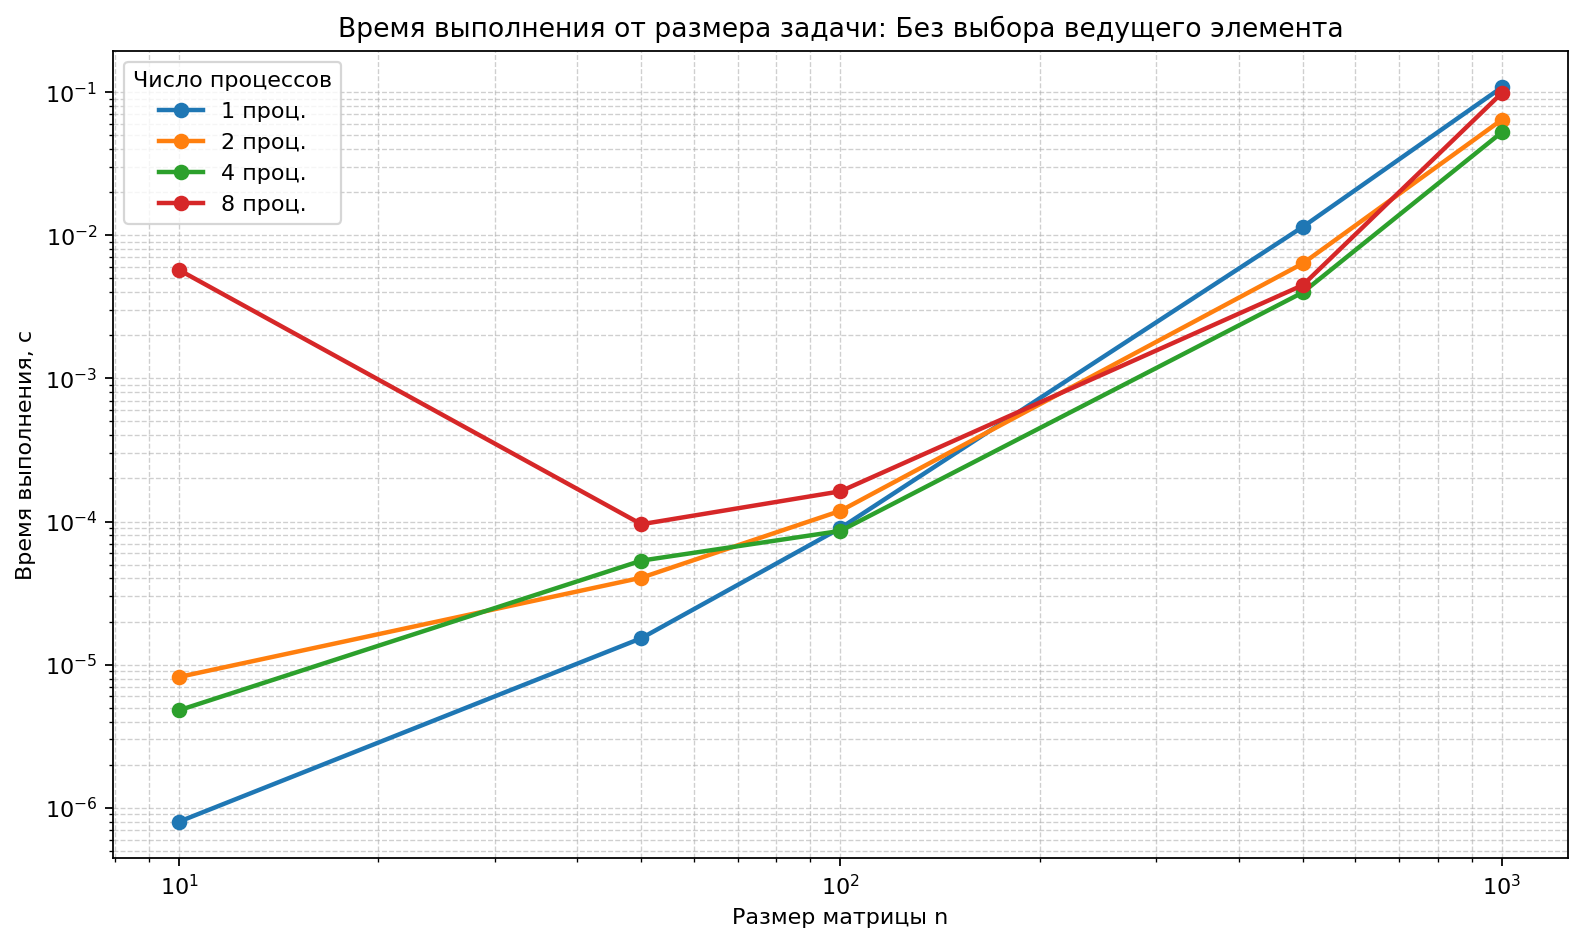
\includegraphics[width=\linewidth]{runtime_vs_n_no.png}
        \caption{Без выбора}
    \end{subfigure}
    \begin{subfigure}{0.48\textwidth}
        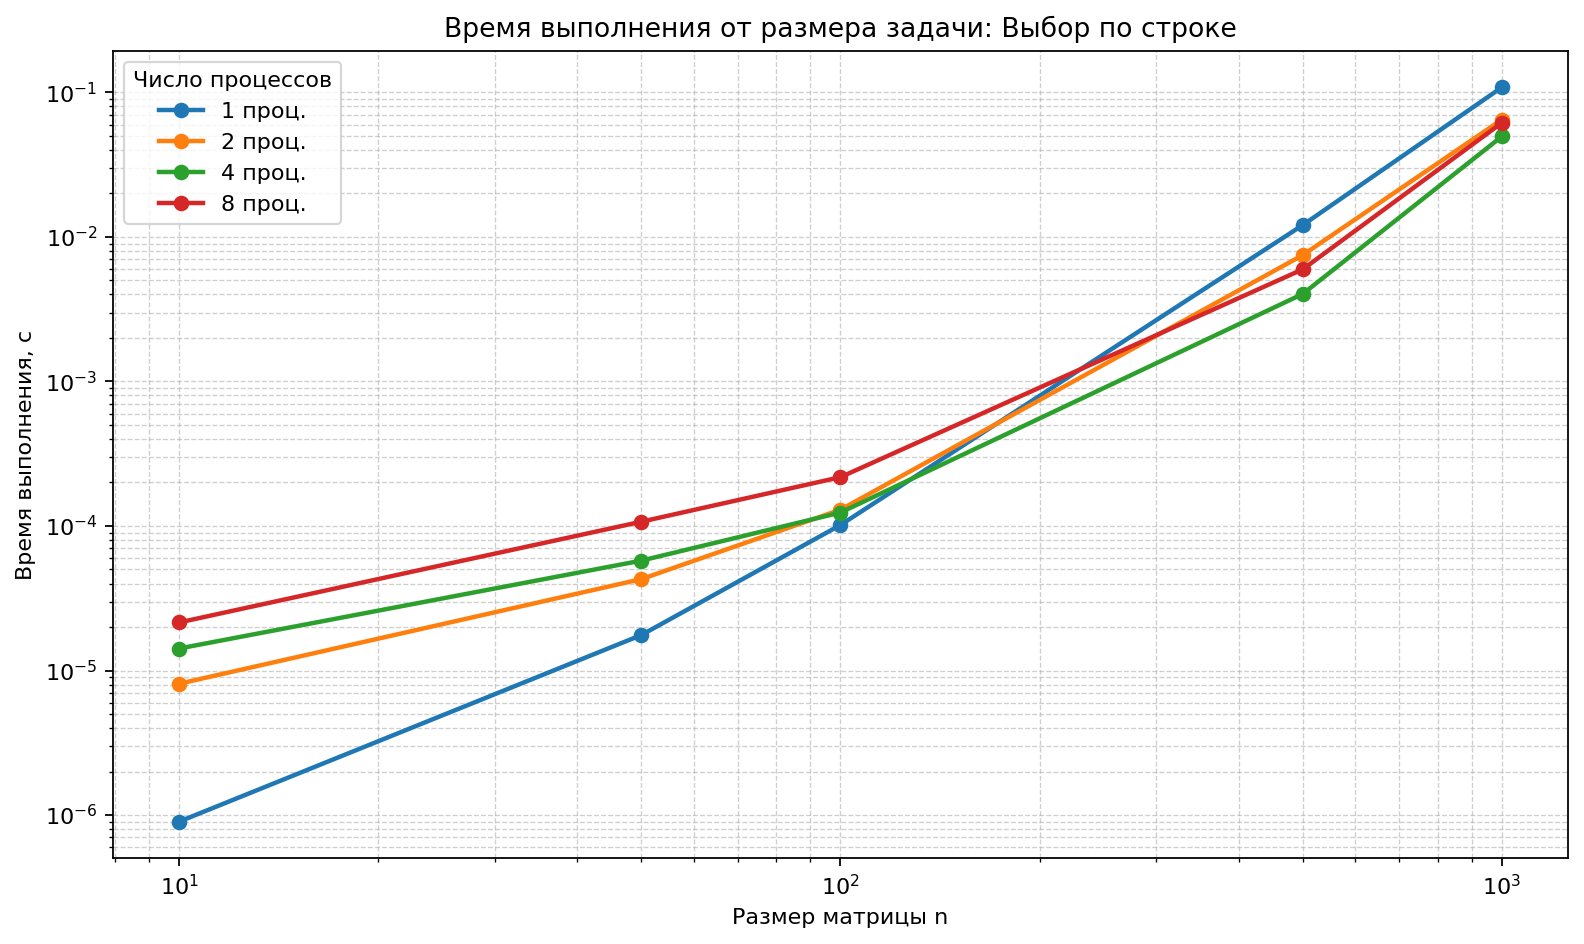
\includegraphics[width=\linewidth]{runtime_vs_n_row.png}
        \caption{Выбор по строке}
    \end{subfigure}
    \begin{subfigure}{0.48\textwidth}
        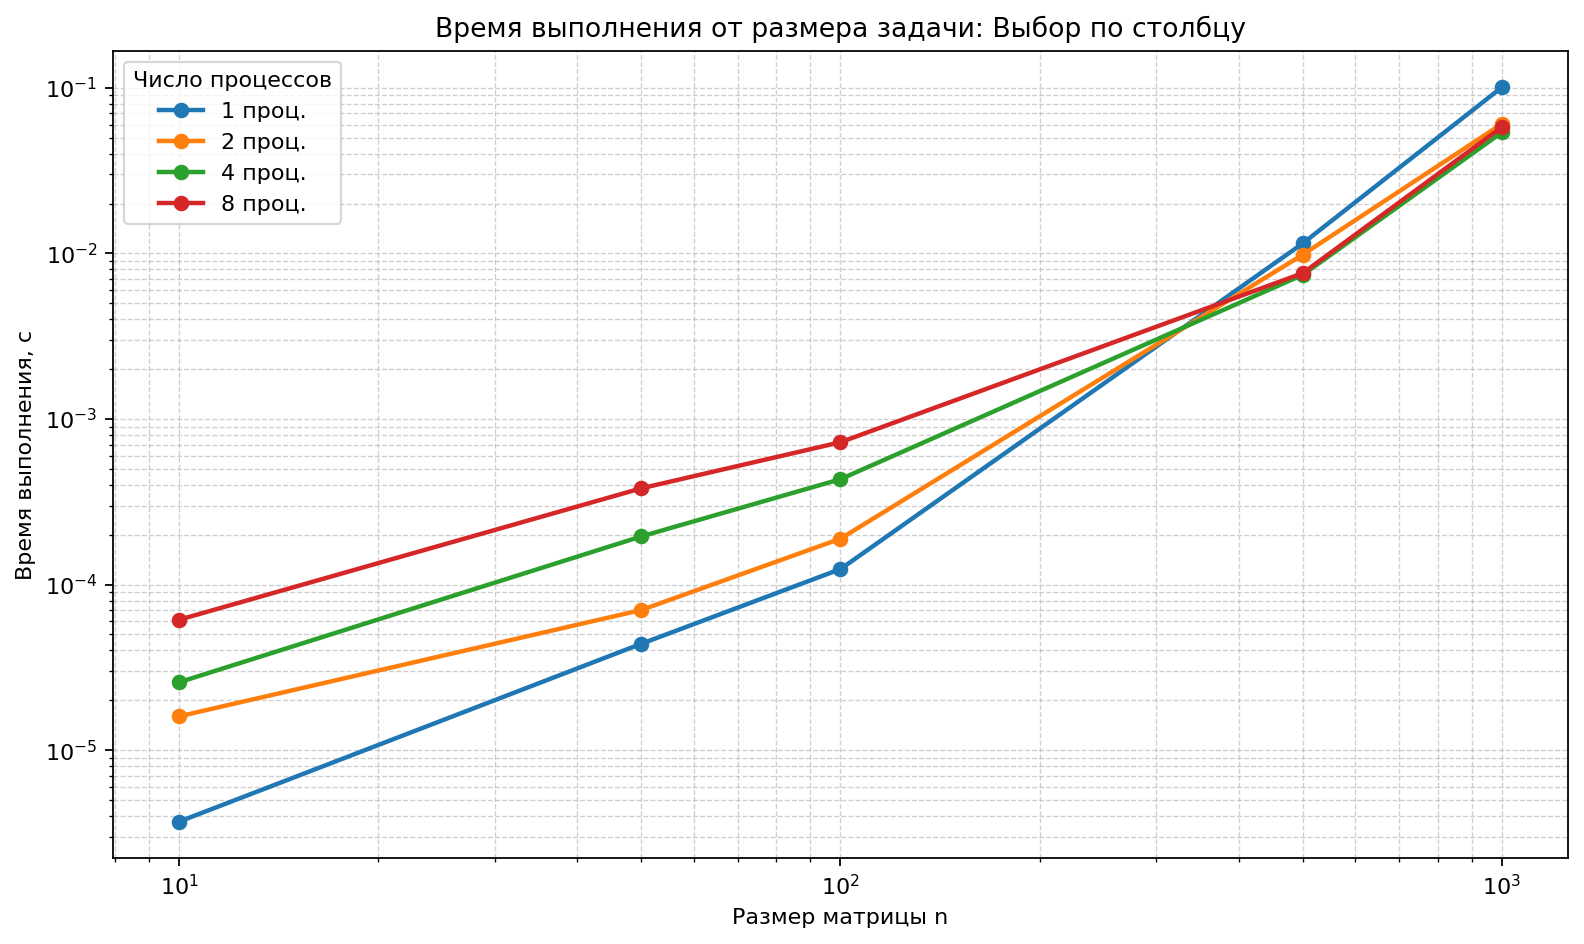
\includegraphics[width=\linewidth]{runtime_vs_n_column.png}
        \caption{Выбор по столбцу}
    \end{subfigure}
    \begin{subfigure}{0.48\textwidth}
        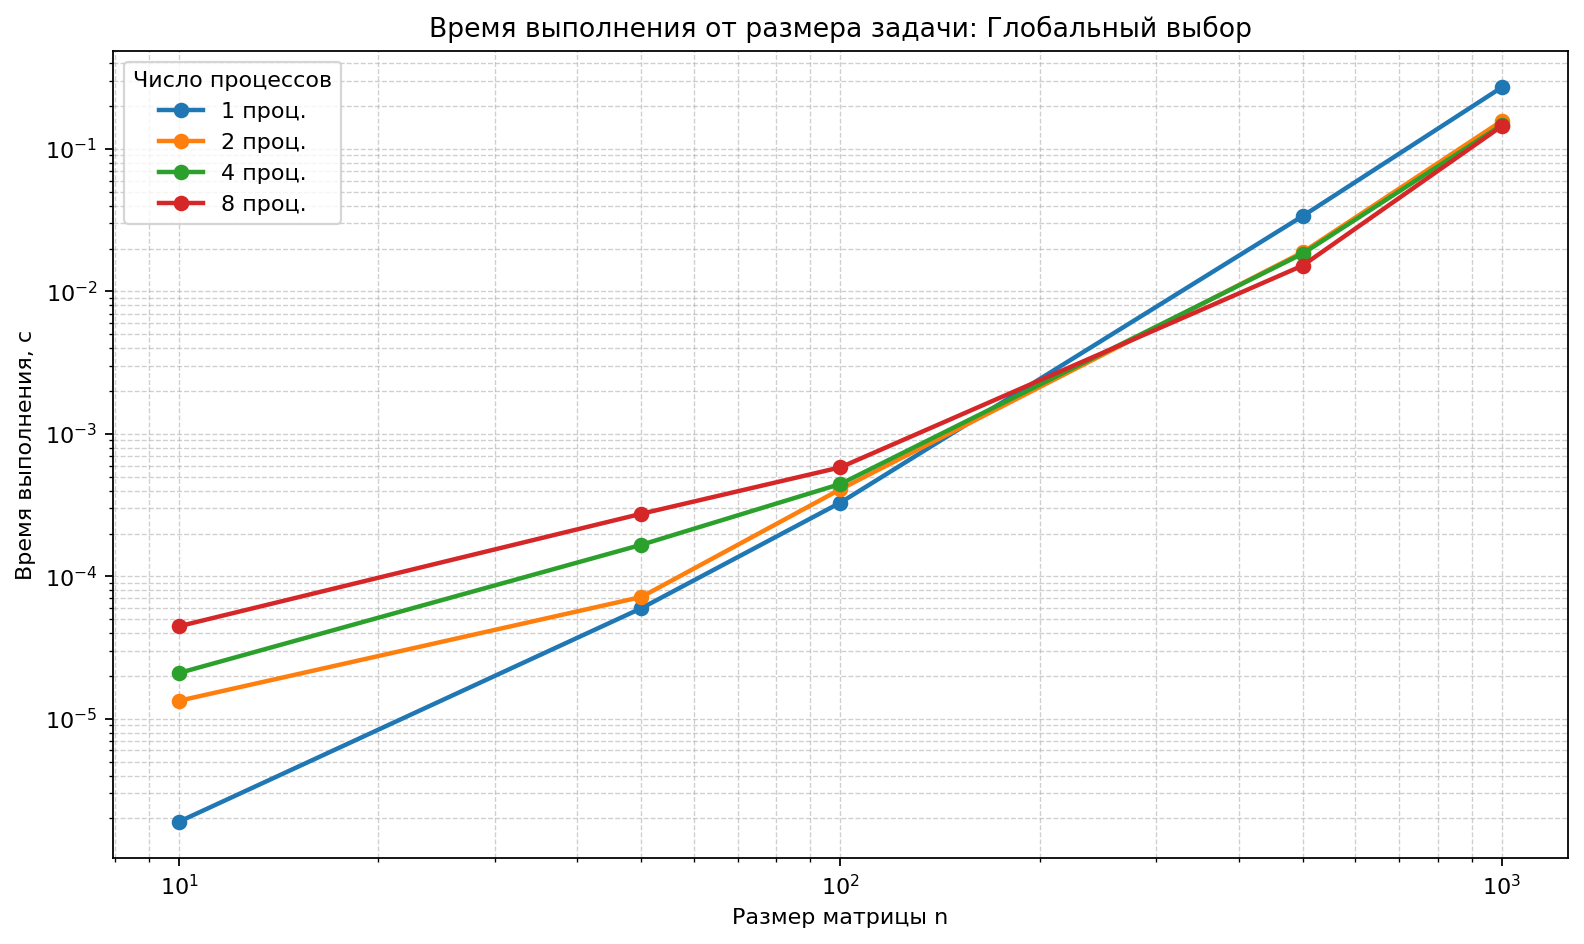
\includegraphics[width=\linewidth]{runtime_vs_n_global.png}
        \caption{Глобальный выбор}
    \end{subfigure}
    \caption{Зависимость времени выполнения от размера матрицы.}
\end{figure}

\subsection{Ускорение от размера задачи}

\begin{figure}[H]
    \centering
    \begin{subfigure}{0.48\textwidth}
        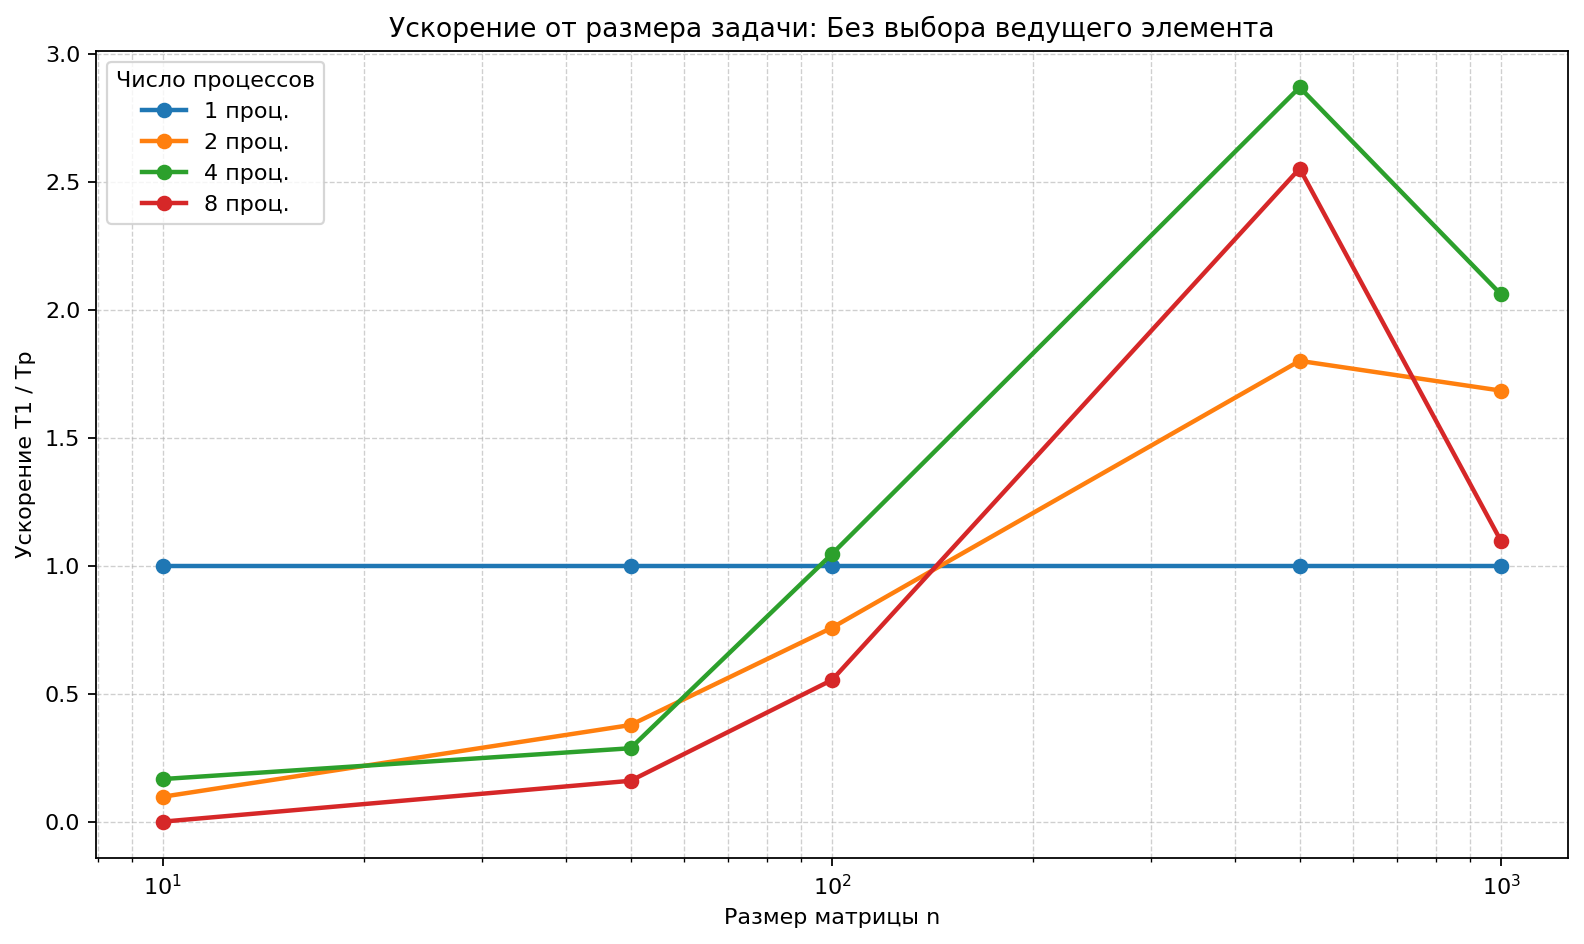
\includegraphics[width=\linewidth]{speedup_vs_n_no.png}
        \caption{Без выбора}
    \end{subfigure}
    \begin{subfigure}{0.48\textwidth}
        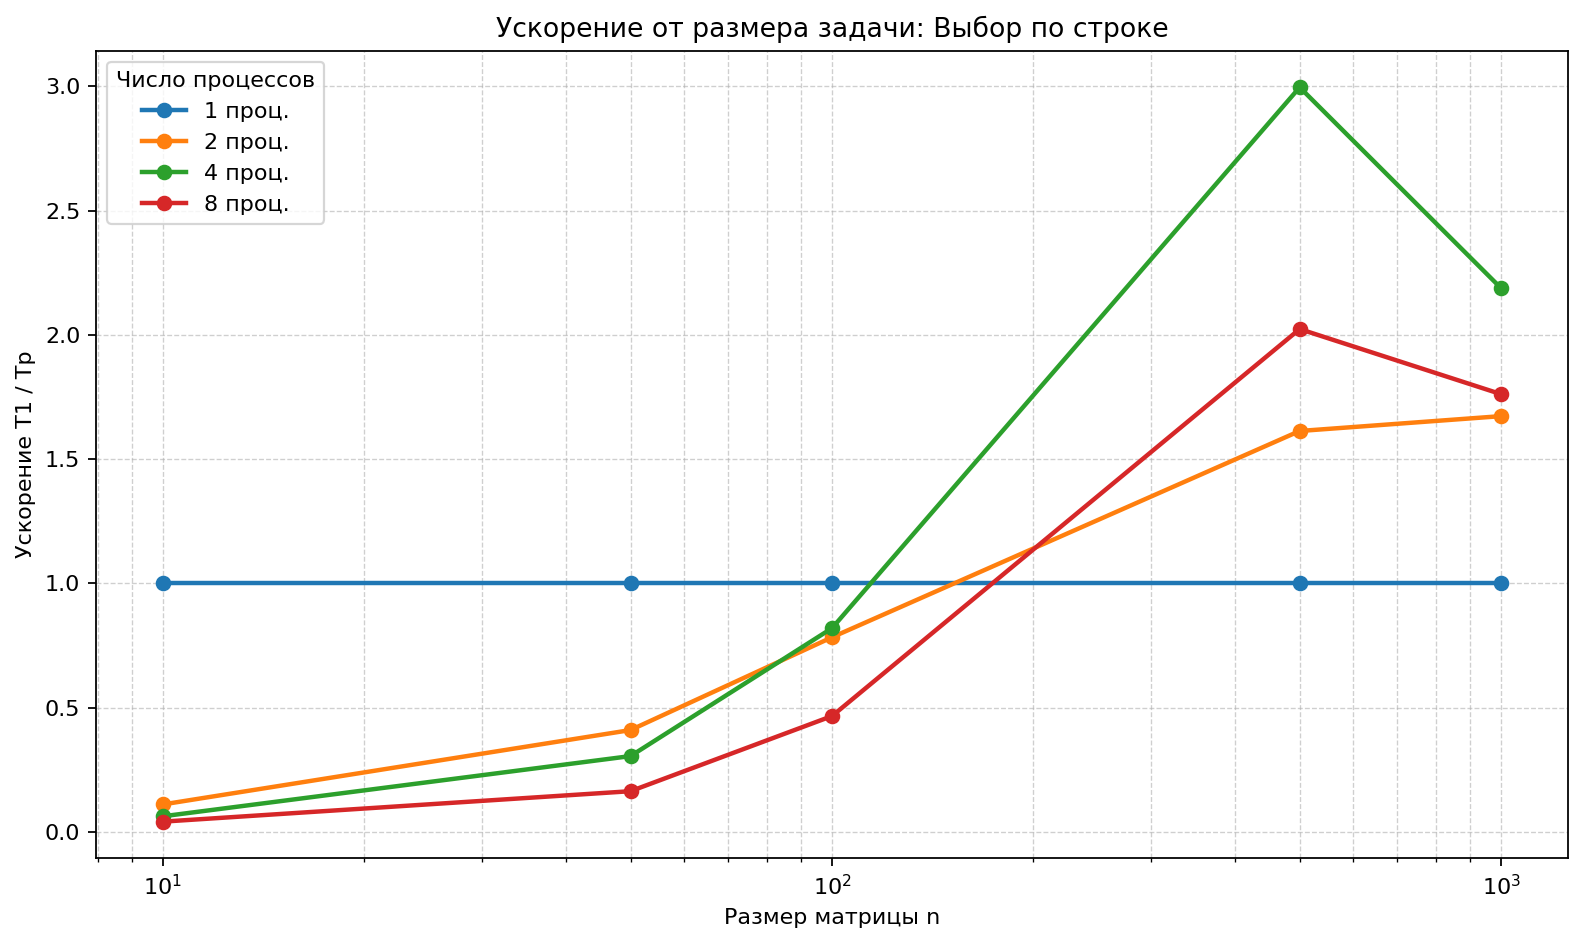
\includegraphics[width=\linewidth]{speedup_vs_n_row.png}
        \caption{Выбор по строке}
    \end{subfigure}
    \begin{subfigure}{0.48\textwidth}
        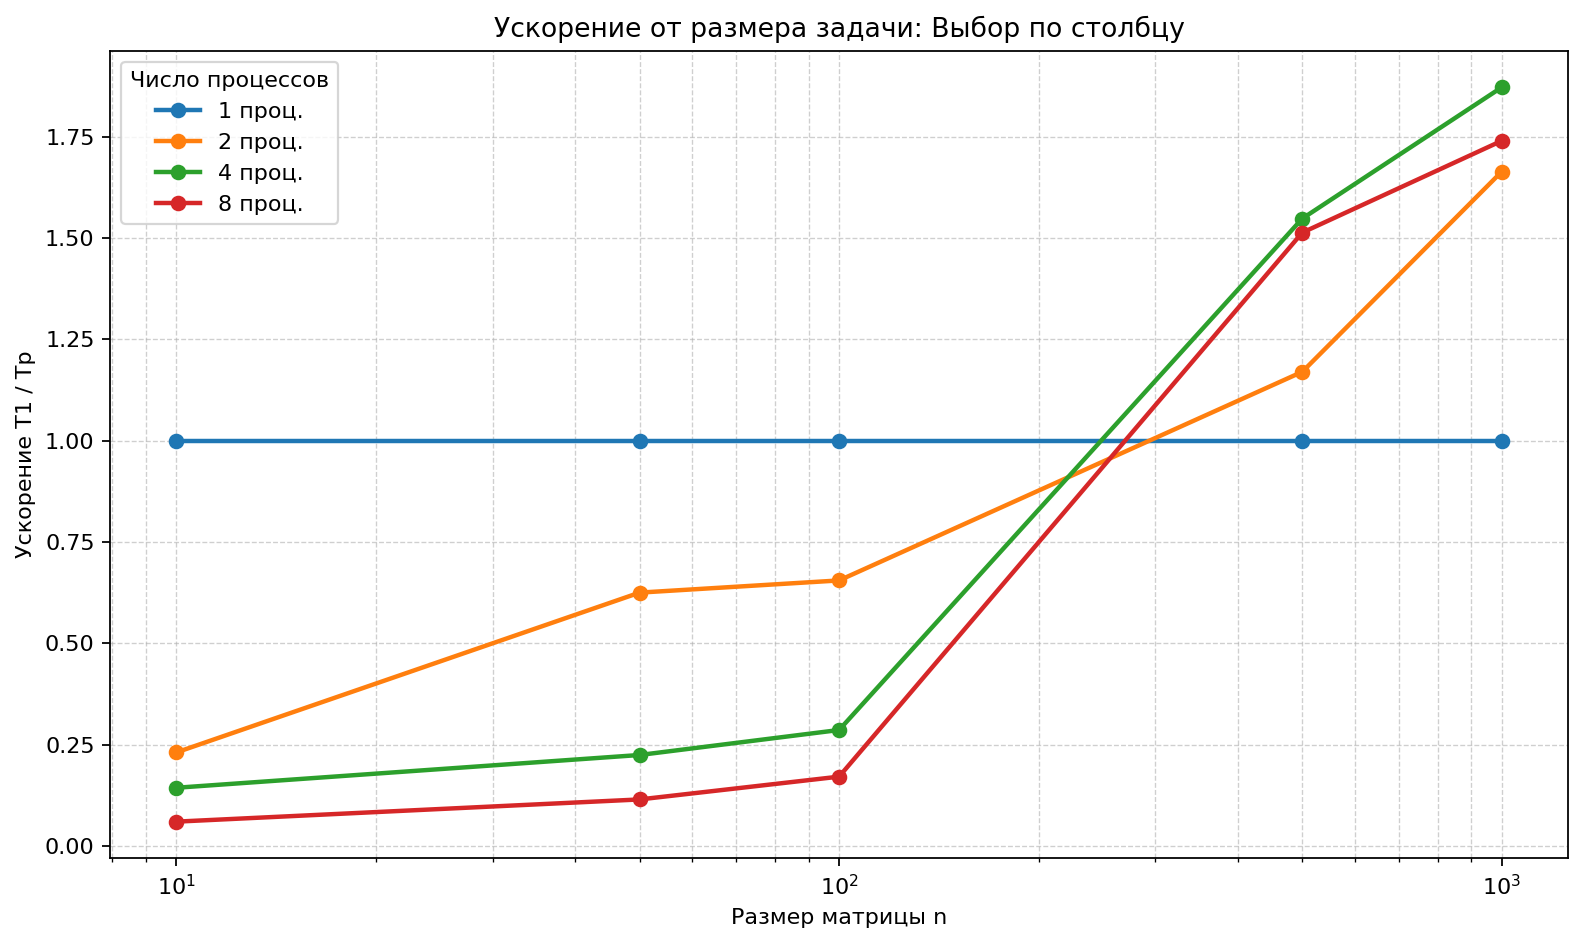
\includegraphics[width=\linewidth]{speedup_vs_n_column.png}
        \caption{Выбор по столбцу}
    \end{subfigure}
    \begin{subfigure}{0.48\textwidth}
        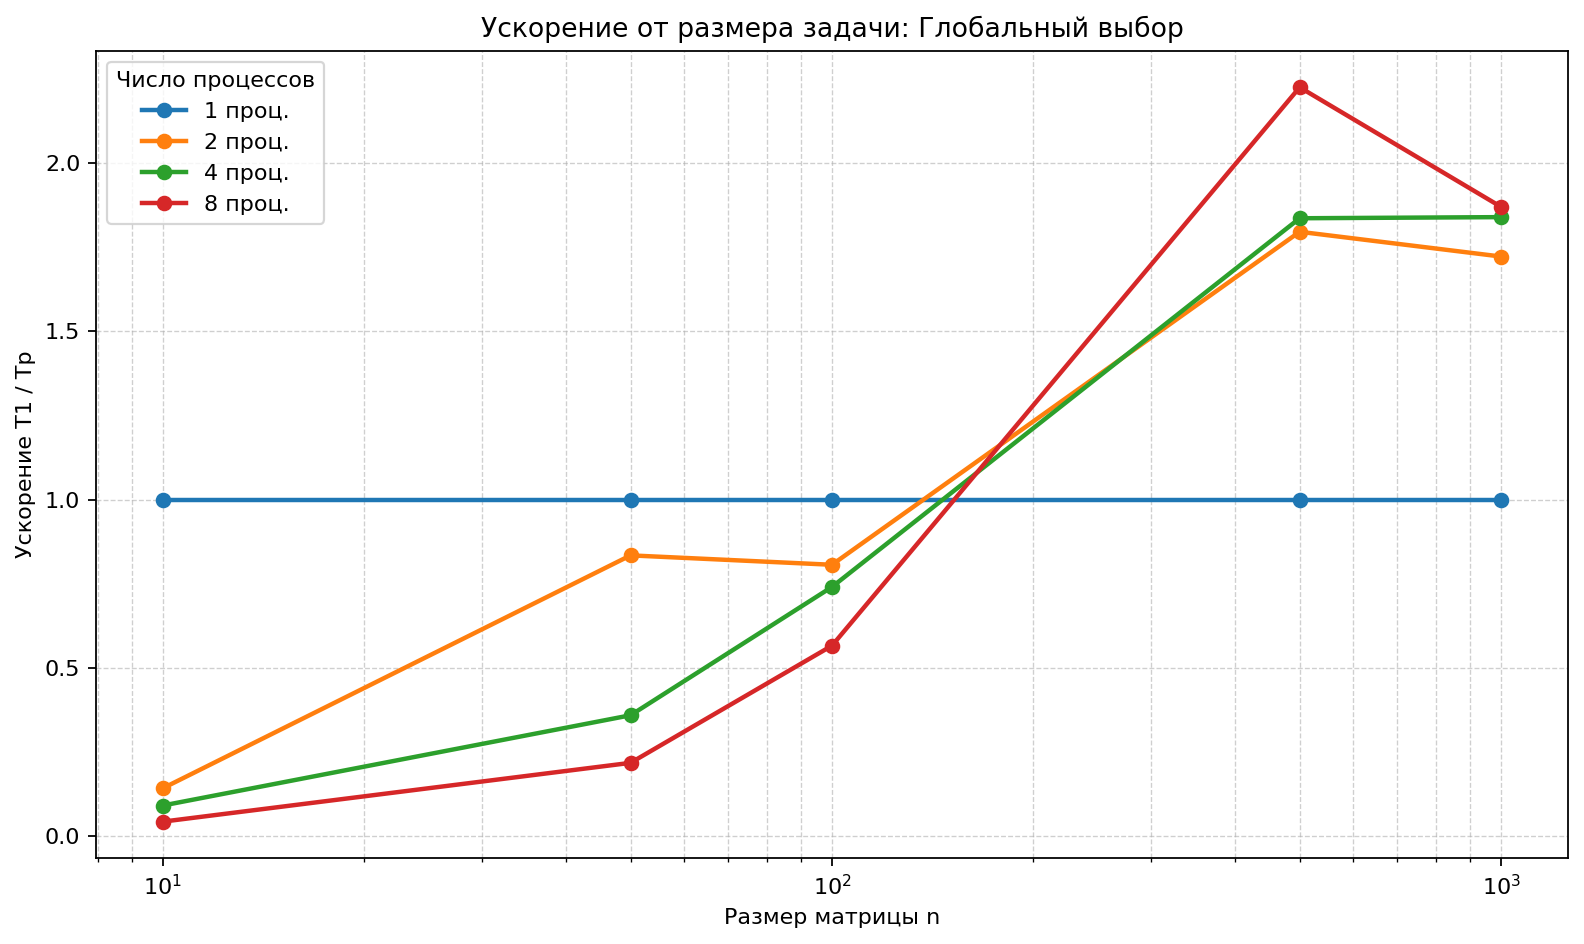
\includegraphics[width=\linewidth]{speedup_vs_n_global.png}
        \caption{Глобальный выбор}
    \end{subfigure}
    \caption{Зависимость ускорения от размера матрицы.}
\end{figure}

\subsection{Время выполнения от числа процессов}

\begin{figure}[H]
    \centering
    \begin{subfigure}{0.48\textwidth}
        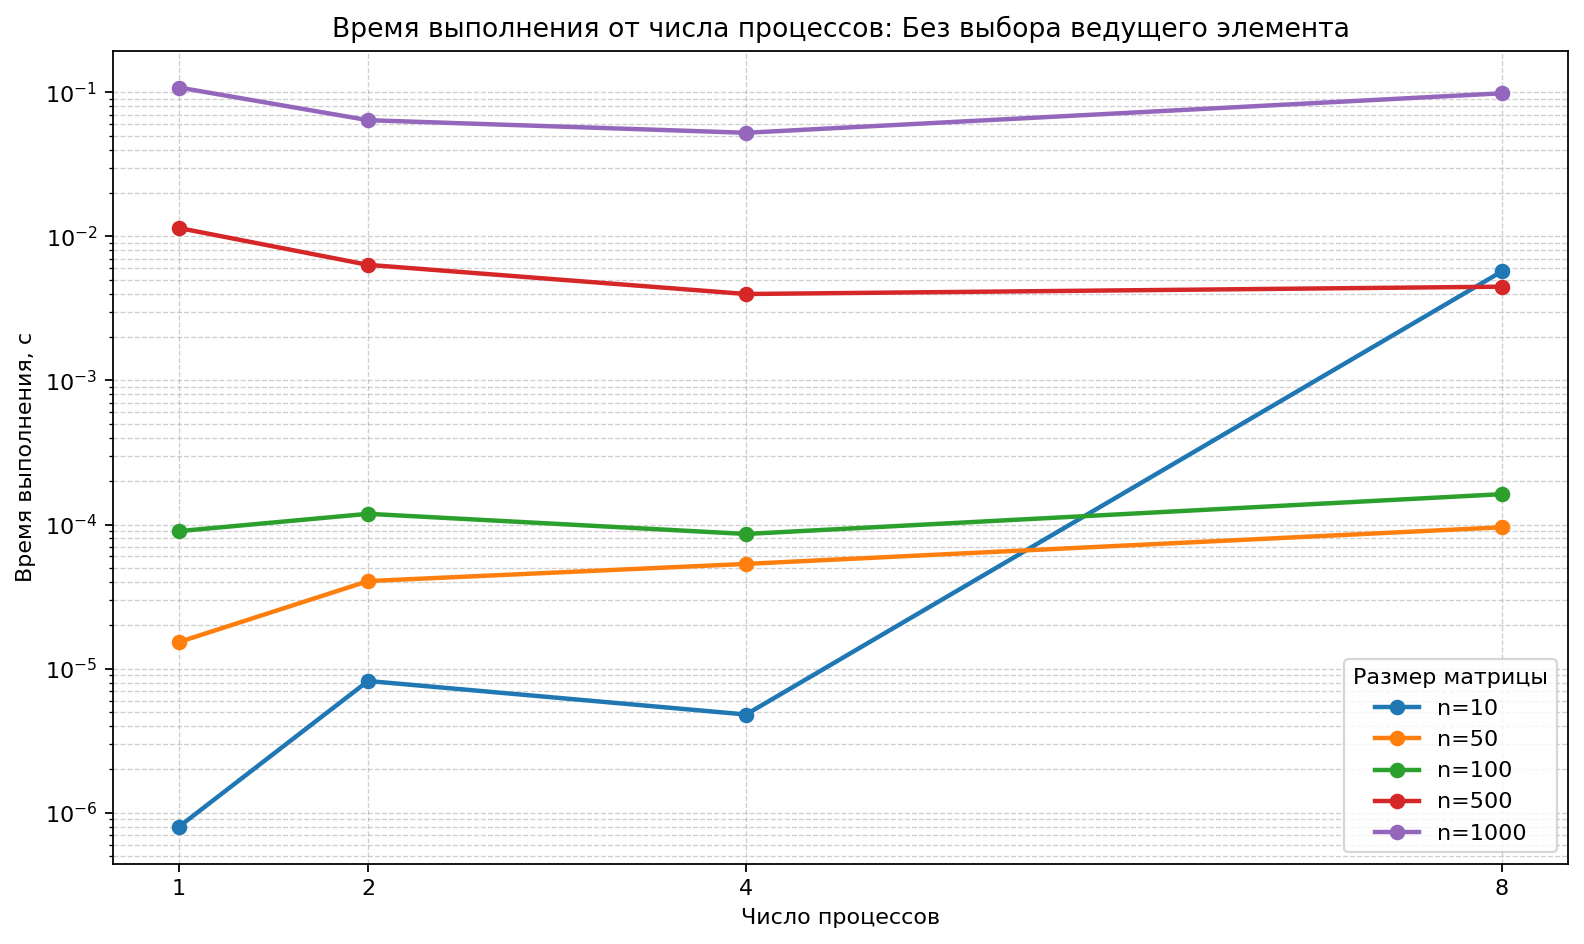
\includegraphics[width=\linewidth]{runtime_vs_procs_no.png}
        \caption{Без выбора}
    \end{subfigure}
    \begin{subfigure}{0.48\textwidth}
        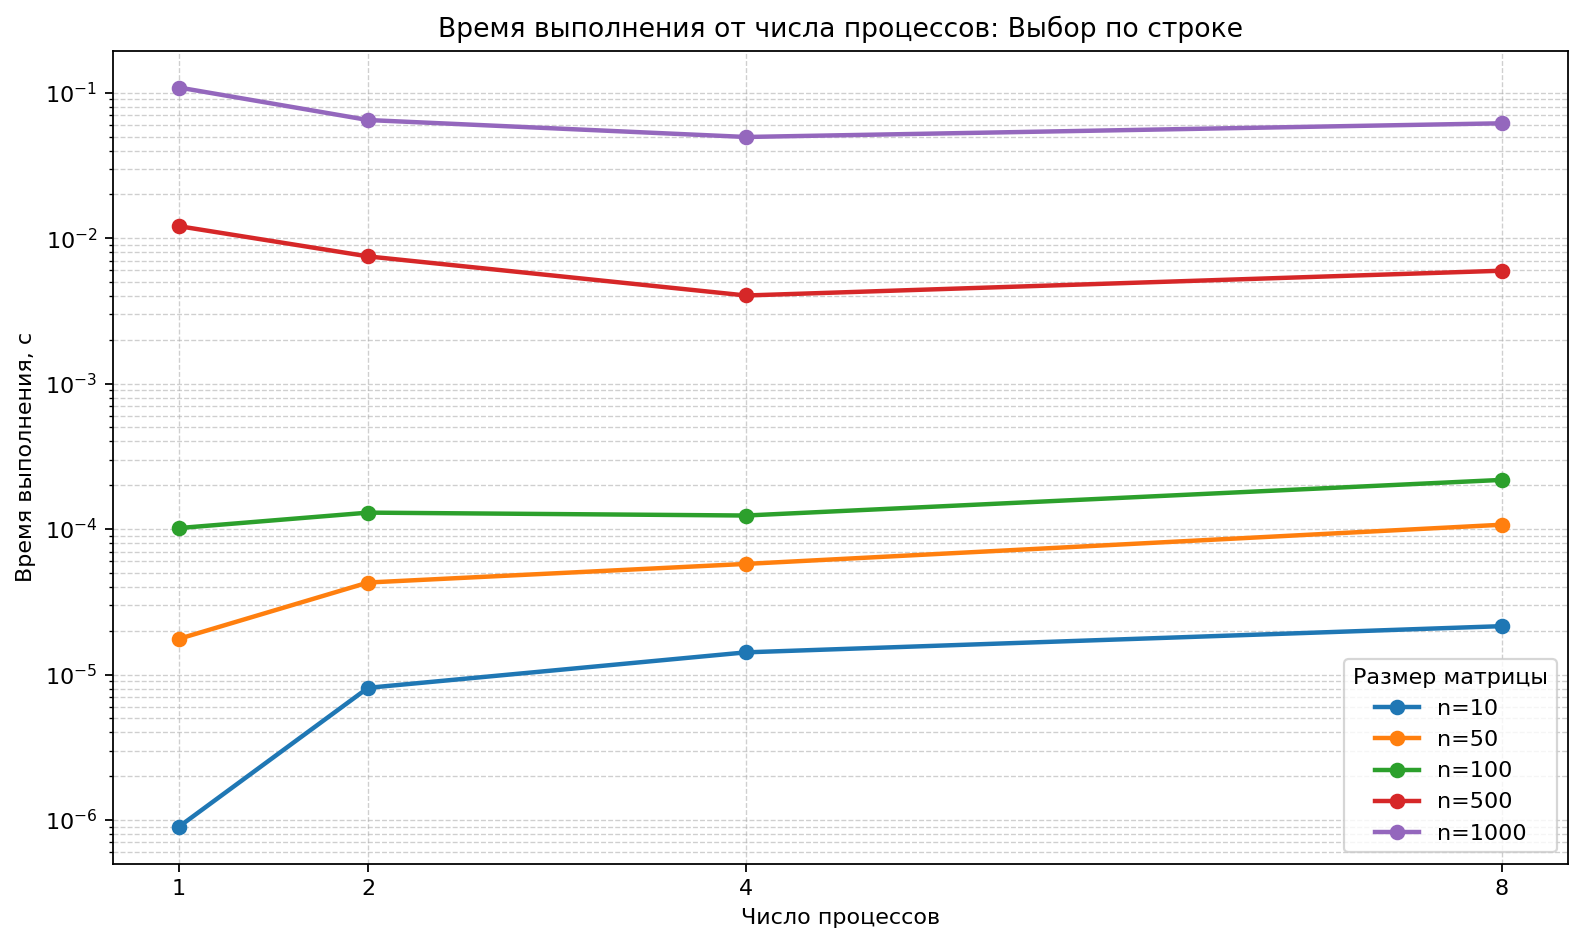
\includegraphics[width=\linewidth]{runtime_vs_procs_row.png}
        \caption{Выбор по строке}
    \end{subfigure}
    \begin{subfigure}{0.48\textwidth}
        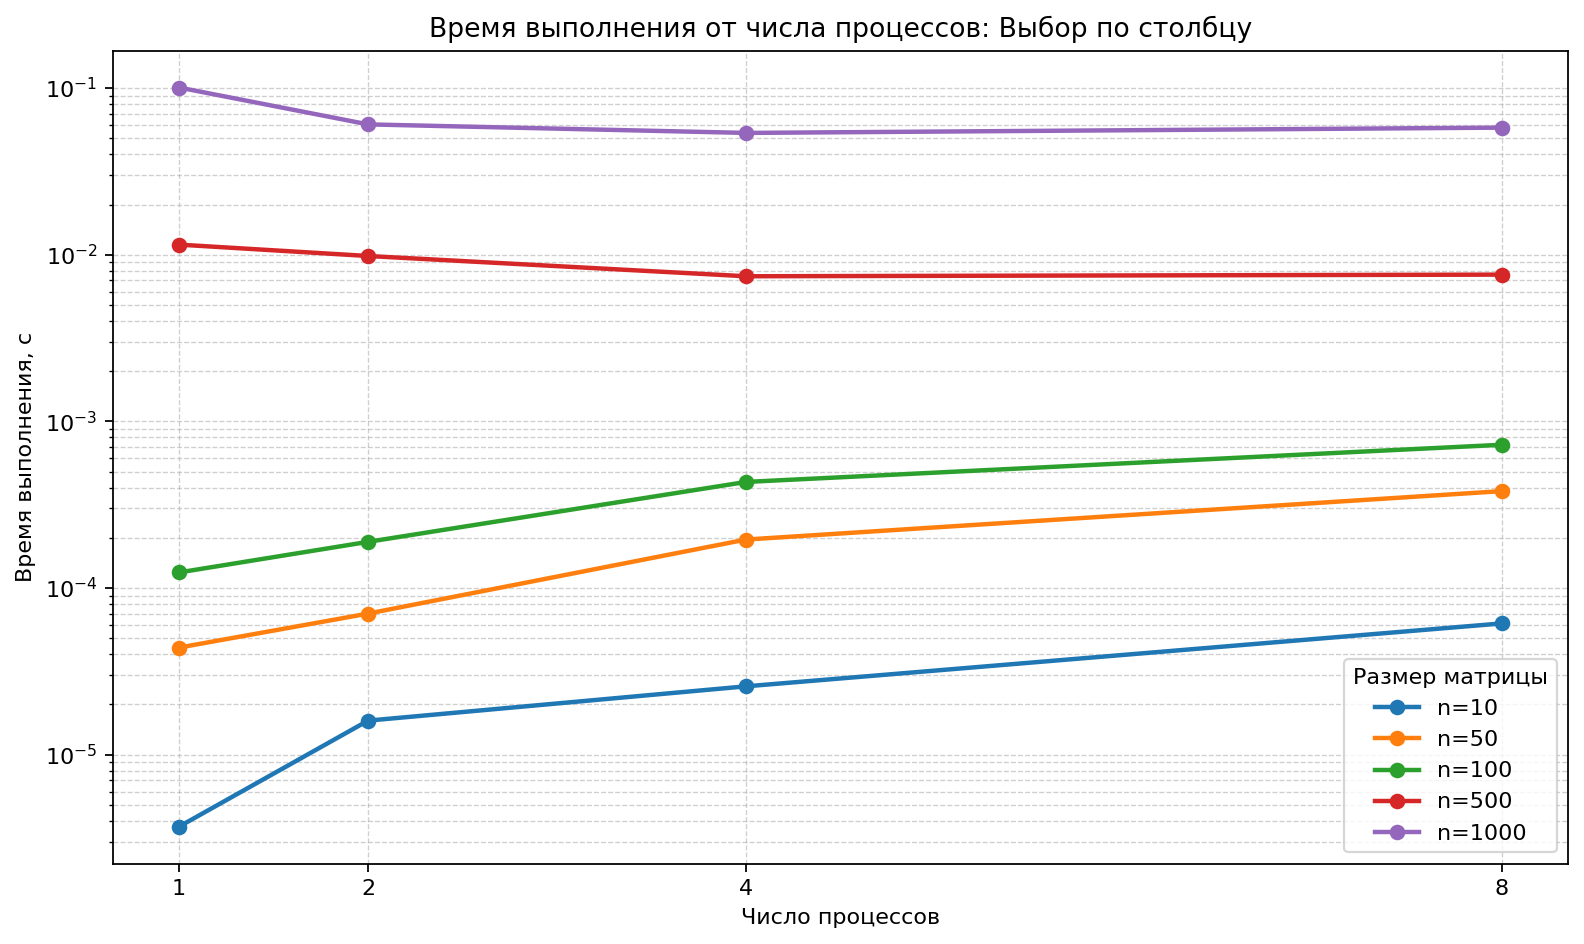
\includegraphics[width=\linewidth]{runtime_vs_procs_column.png}
        \caption{Выбор по столбцу}
    \end{subfigure}
    \begin{subfigure}{0.48\textwidth}
        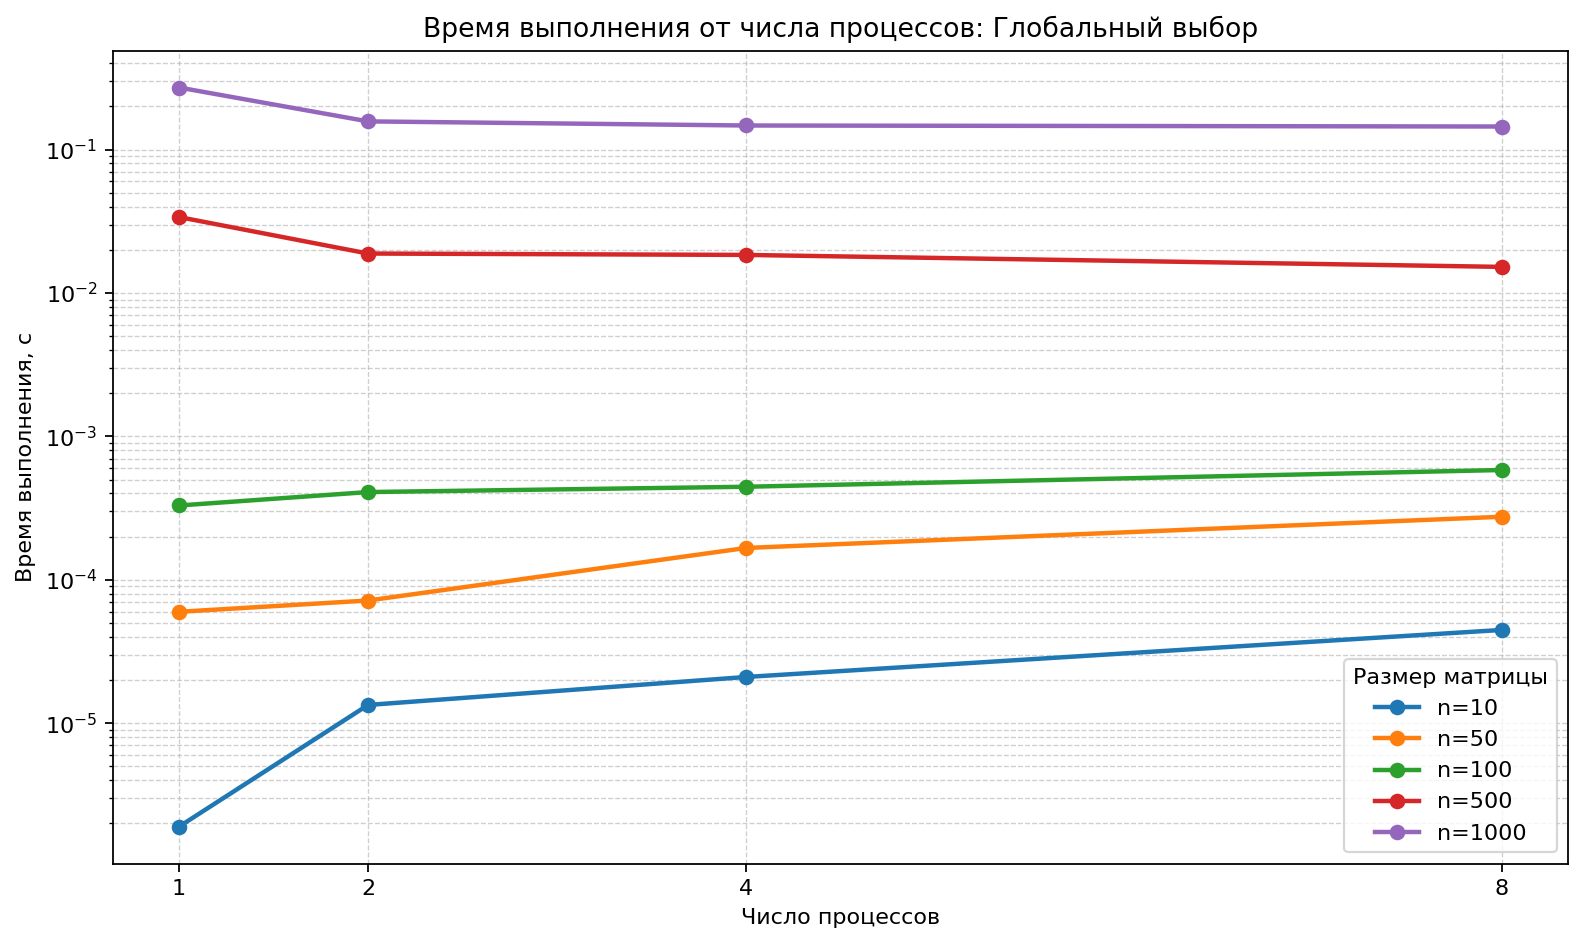
\includegraphics[width=\linewidth]{runtime_vs_procs_global.png}
        \caption{Глобальный выбор}
    \end{subfigure}
    \caption{Зависимость времени выполнения от числа MPI-процессов.}
\end{figure}

\subsection{Точность}

\begin{figure}[H]
    \centering
    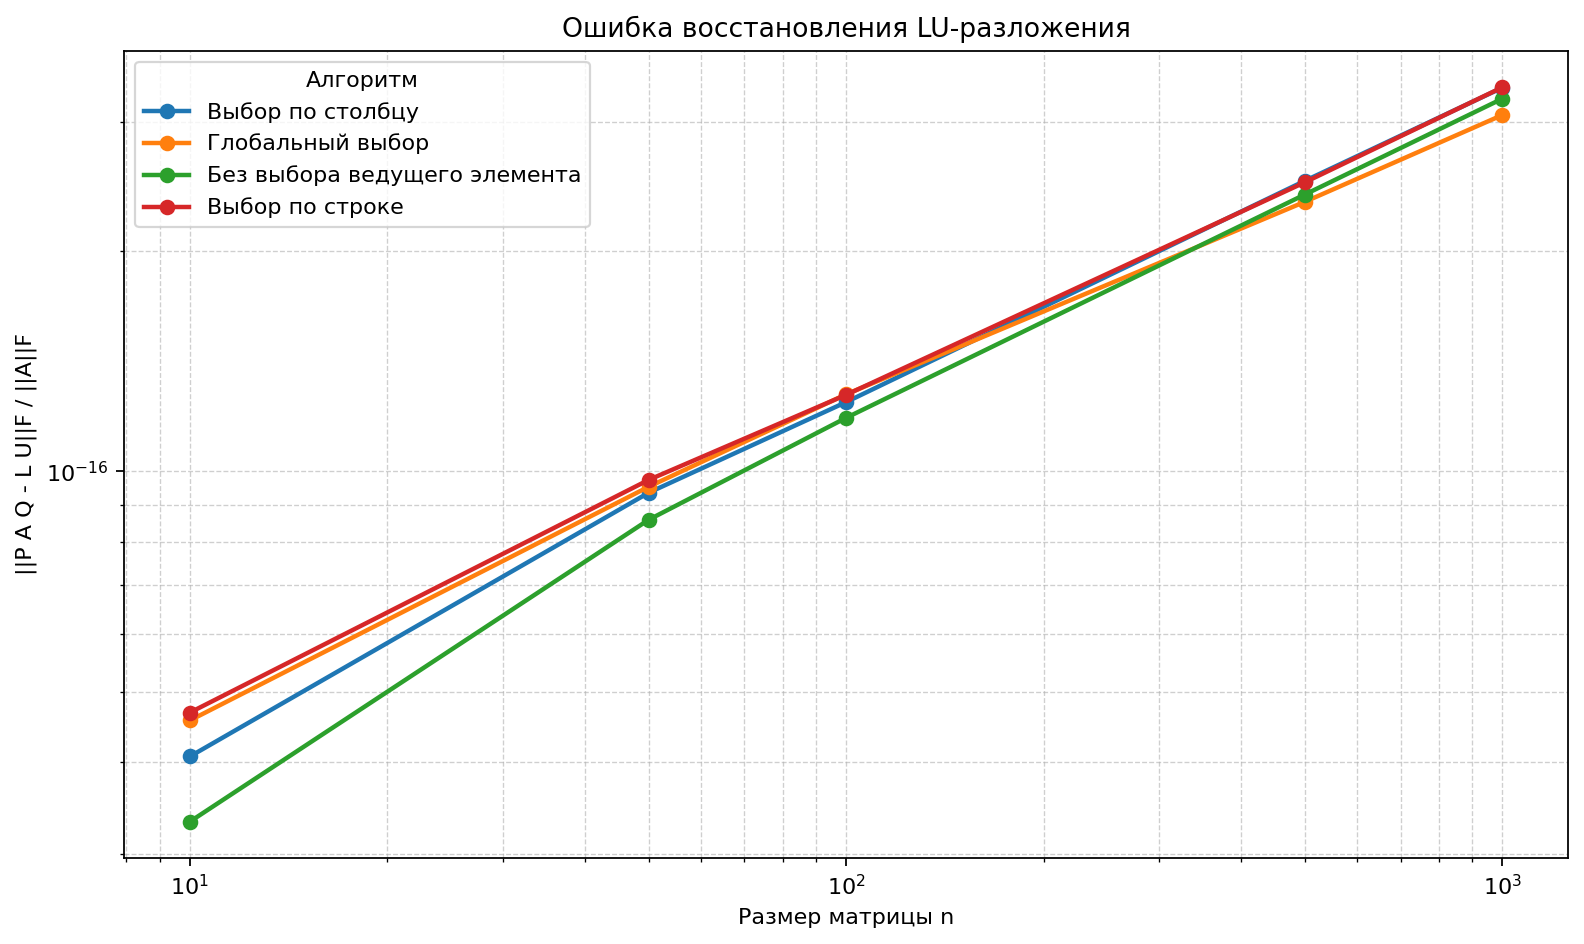
\includegraphics[width=0.85\textwidth]{reconstruction_error_vs_n.png}
    \caption{Ошибка восстановления LU-разложения.}
\end{figure}

\begin{figure}[H]
    \centering
    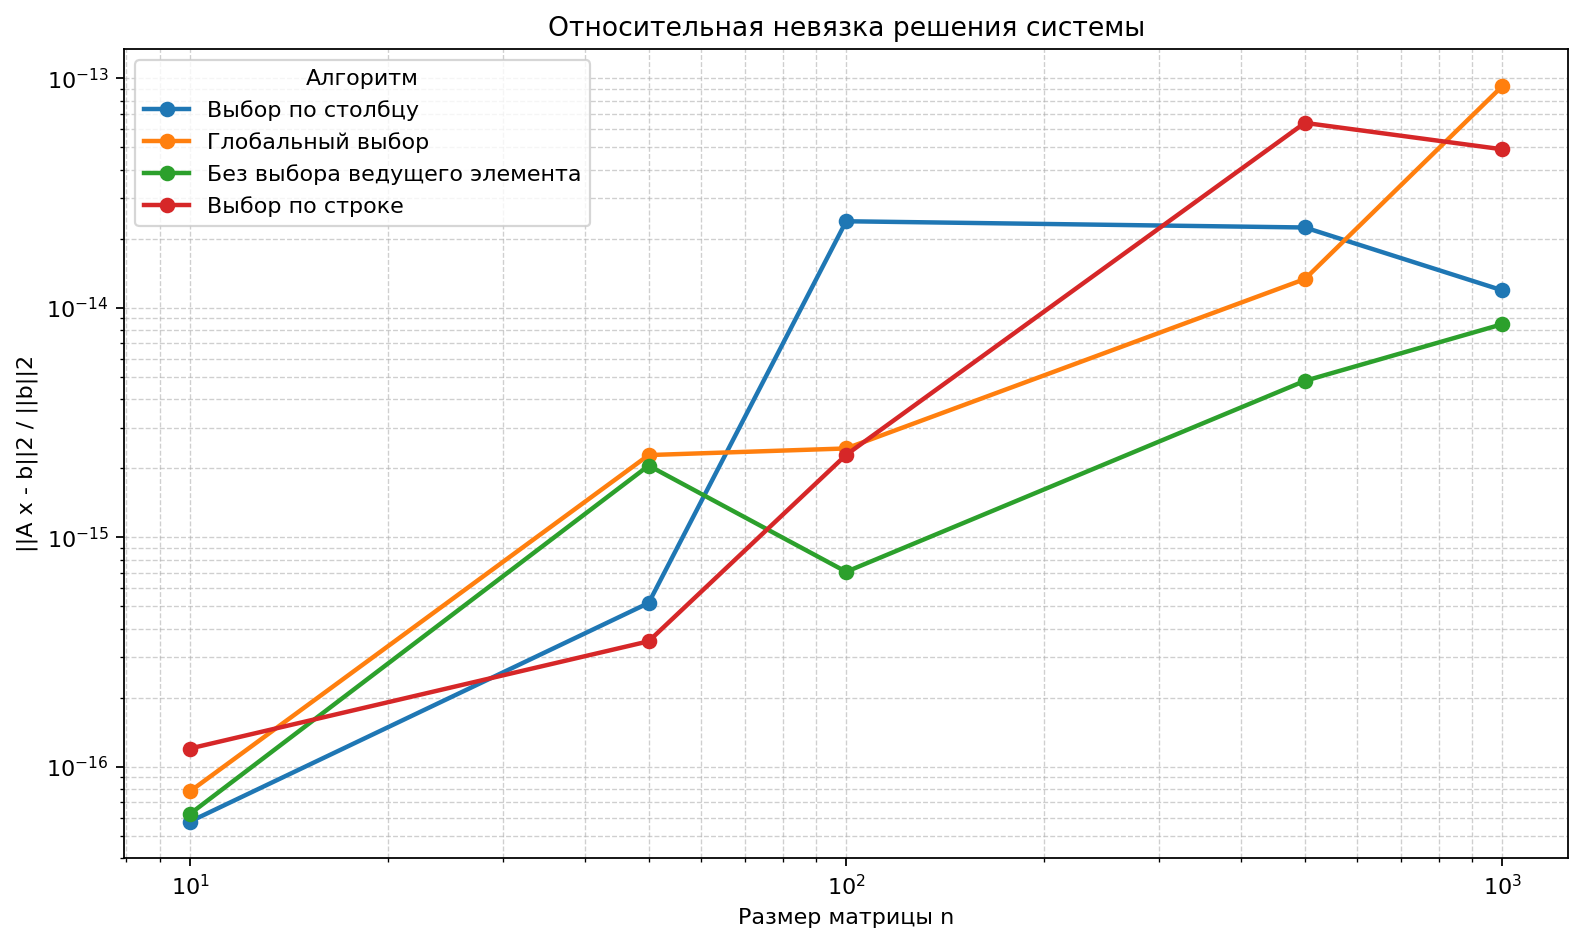
\includegraphics[width=0.85\textwidth]{residual_vs_n.png}
    \caption{Относительная невязка решения тестовой системы.}
\end{figure}

\section{Анализ времени выполнения}

Время выполнения возрастает с увеличением $n$, что соответствует вычислительной сложности LU-разложения порядка $O(n^3)$. Для малых размеров матрицы накладные расходы MPI, включая рассылку ведущей строки и синхронизацию процессов, сравнимы с объемом полезных вычислений. Поэтому при $n=10$ и $n=50$ увеличение числа процессов часто не приводит к ускорению и может даже увеличивать время выполнения.

Для больших матриц полезная вычислительная нагрузка становится существеннее. По данным для $n=1000$ медианные времена для режима без выбора составили $0.108050$ с на одном процессе, $0.064124$ с на двух процессах, $0.052428$ с на четырех процессах и $0.098542$ с на восьми процессах. Для выбора по строке соответствующие времена составили $0.108554$, $0.064886$, $0.049623$ и $0.061631$ с. Это показывает, что распараллеливание становится заметнее на крупных задачах, однако масштабирование ограничивается коммуникациями и дисбалансом объема работы на поздних шагах разложения.

\section{Анализ ускорения и эффективности}

Максимальные наблюдаемые ускорения составили: $2.871$ для режима без выбора ведущего элемента, $2.996$ для выбора по строке, $1.872$ для выбора по столбцу и $2.226$ для глобального выбора. Значения ускорения меньше идеального $S_p=p$, что является ожидаемым результатом для распределенной реализации с регулярными коллективными обменами.

Эффективность $E_p$ уменьшается при росте числа процессов, особенно на малых матрицах. Это объясняется тем, что время коммуникаций и синхронизаций начинает занимать большую долю общего времени. Кроме того, на последних шагах LU-разложения активная подматрица уменьшается, поэтому часть процессов получает меньше работы, а относительная стоимость обменов возрастает.

\section{Анализ точности на матрице Гильберта}

Матрица Гильберта плохо обусловлена, поэтому даже при малых ошибках восстановления разложения невязка решения может расти с увеличением $n$. В проведенных экспериментах ошибка восстановления находилась примерно на уровне $10^{-17}$--$10^{-16}$, а относительная невязка для больших размеров достигала порядка $10^{-14}$--$10^{-13}$.

Выбор ведущего элемента повышает численную устойчивость алгоритма, поскольку позволяет избегать деления на слишком малые элементы и уменьшает рост элементов в процессе исключения. При этом разные стратегии перестановок влияют на точность по-разному: выбор по строке переставляет столбцы, выбор по столбцу переставляет строки, а глобальный выбор использует обе перестановки и является наиболее полным вариантом с точки зрения поиска крупного ведущего элемента.

Однако повышение устойчивости достигается ценой дополнительных коммуникационных расходов. Для выбора по столбцу требуется параллельный поиск максимума в столбце и, при необходимости, обмен строками между процессами. Для глобального выбора требуется поиск максимума во всей активной подматрице и возможны как обмен строк, так и перестановка столбцов. Поэтому pivoting обычно улучшает численную надежность, но увеличивает время на коммуникации, особенно при большом числе процессов и небольших размерах матрицы.

\section{Вывод}

В ходе лабораторной работы была реализована MPI-программа LU-разложения матрицы Гильберта с четырьмя вариантами выбора ведущего элемента: без выбора, выбор по строке, выбор по столбцу и глобальный выбор. Для распределения данных использовалась циклическая схема владения строками $owner(i)=i \bmod p$, а ведущая строка передавалась процессам через MPI.

Экспериментальные результаты показали, что параллельное выполнение становится полезным преимущественно на больших размерах матрицы. На малых задачах накладные расходы MPI превосходят выигрыш от распараллеливания. Максимальные ускорения оказались ниже идеальных из-за коммуникаций, синхронизаций и уменьшения активной подматрицы на поздних шагах алгоритма.

Методы выбора ведущего элемента улучшают устойчивость вычислений на плохо обусловленной матрице Гильберта, однако требуют дополнительных обменов и глобальных редукций. Таким образом, выбор стратегии pivoting является компромиссом между точностью и коммуникационной стоимостью параллельного алгоритма.

\end{document}
